\documentclass{ltjsarticle}
%\usepackage[dvipdfmx]{graphicx}
\usepackage{graphicx}
\usepackage{booktabs}
\usepackage{mathcomp}
\usepackage{array}
\usepackage{mathtools,amssymb}
\usepackage{siunitx}
\usepackage{multirow}
\usepackage{tabularx}
\usepackage{subcaption}
\usepackage{float}
\usepackage{setspace}
\usepackage{abstract}


\title{仮想筋電義手の開発に関する研究}
\author{河合 将暉}
\adviser{戸崎 哲也}

\thispagestyle{empty}
\pagestyle{empty}

\begin{document}
\maketitle

\section{はじめに}
	上肢切断者が筋電義手を装着する際,自在に扱うことができるように
	訓練を行う必要がある.VRを用いた筋電義手トレーニングの効果につ
	いては先行研究\cite{ref:1}\cite{ref:2}で検討されており,本研究
	では仮想筋電義手モデルの見た目の違いによる訓練効果や幻肢痛緩
	和の効果について着目し3Dスキャナで取り込んだ仮想筋電義手モデル
	を用いたVRトレーニングシステムの構成を目的とする.
	\vspace{-10pt}

\section{研究内容}
	\subsection{3Dモデルの構成}
		本研究では仮想筋電義手のモデルをリアルにする手段として, 3D
		スキャナ ``EinScan HX''を用いて左腕の肘から手先までをスキャン
		して取得した3Dモデルをblenderで表面のノイズ部分を除去・補正し
		見た目に違和感のない程度に後処理を行った.そしてそのモデルに対して
		3Dモデルの動きを制御するための骨組みであるボーンを図\refeq{fig:VRhand}
		のように配置した.
		\begin{figure}[H]
		\centering
		\begin{minipage}{0.292\columnwidth}
		\centering
		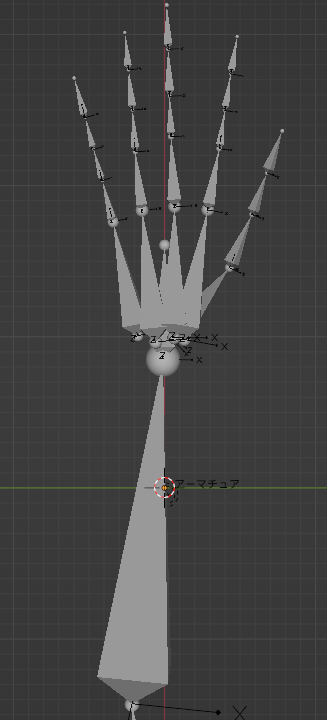
\includegraphics[width = \columnwidth]{figs/handboneLat.png}
		\subcaption{ボーン背面}
		\end{minipage}
		\hspace{0.3pt}
		\begin{minipage}{0.292\columnwidth}
		\centering
		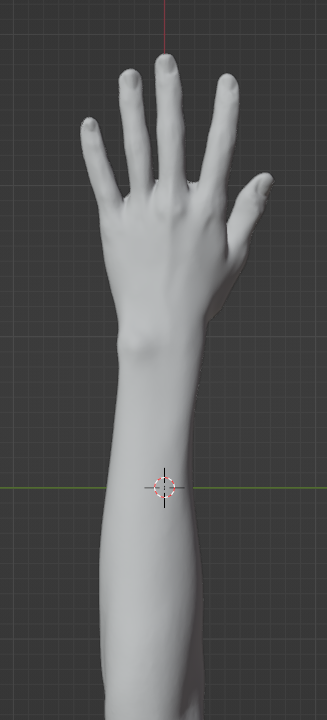
\includegraphics[width = \columnwidth]{figs/handmeshLat.png}
		\subcaption{メッシュ背面}
		\end{minipage}
		\hspace{0.3pt}
		\begin{minipage}{0.292\columnwidth}
		\centering
		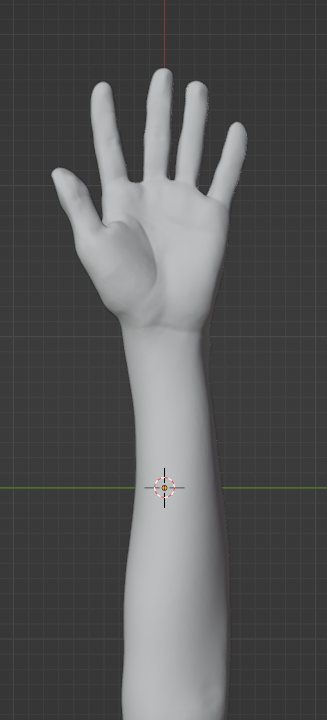
\includegraphics[width = \columnwidth]{figs/handmeshLat_flont.png}
		\subcaption{メッシュ前面}
		\end{minipage}
		\vspace{-10pt}
		\caption{仮想筋電3Dモデル構成図}
		\label{fig:VRhand}
		\end{figure}
		\vspace{-35pt}

	\subsection{VRトレーニングシステムの構成}
		後処理を施した仮想筋電義手モデルを総合開発環境``Unity''に
		インポートし3Dモデルに立体感を与えるため``Reflex Shader2.2''
		を用いてシェーディングを行った.構成したVR空間は研究室の環境上で
		60fpsで動作し,空間上のオブジェクトには物理演算をつけており,
		枠組みの中に動かせるオブジェクトとして球体・立方体・円柱の3Dモデルを,
		固定オブジェクトとして適当な高さの長方形3Dモデルを用意した.Unity
		を用いて構成したVR空間上のオブジェクト配置を図\refeq{fig:gamefield}に示す.

		\begin{figure}[H]
		\centering
		\begin{minipage}{0.521\columnwidth}
		\centering
		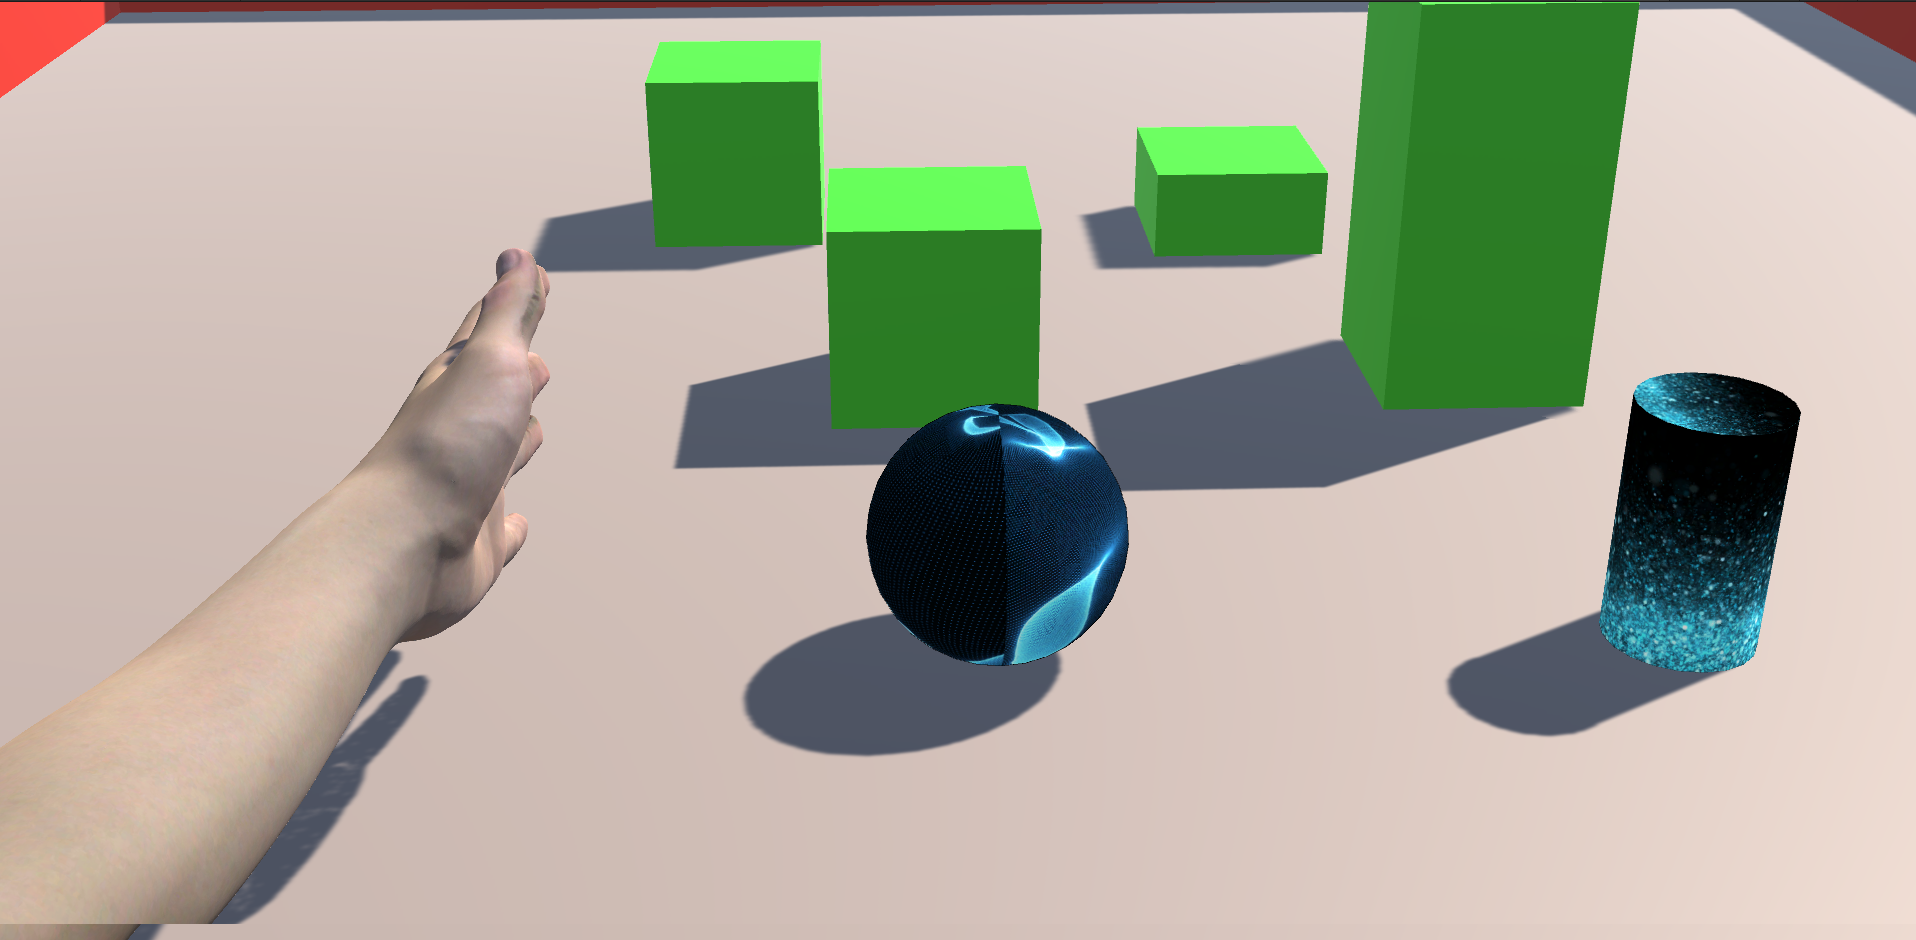
\includegraphics[width = \columnwidth]{figs/gamescreen.png}
		\subcaption{システム稼働時の視点}
		\end{minipage}
		\hspace{0.05\columnwidth}
		\begin{minipage}{0.4\columnwidth}
		\centering
		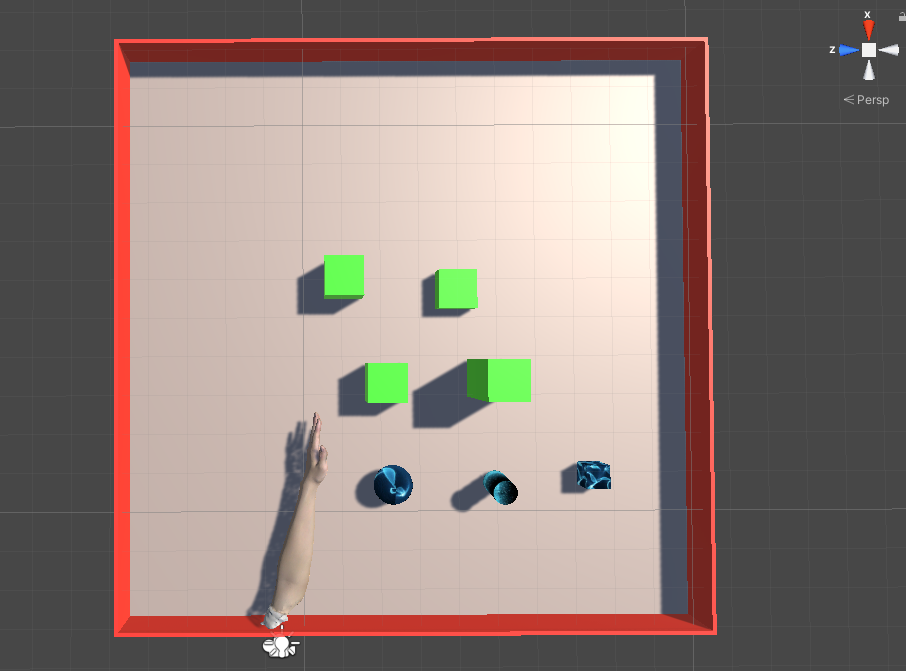
\includegraphics[width = \columnwidth]{figs/fieldup.png}
		\subcaption{上面図}
		\end{minipage}
		\vspace{-10pt}
		\caption{VR空間上のオブジェクト配置図}
		\label{fig:gamefield}
		\end{figure}
		\vspace{-20pt}

		仮想筋電義手モデルはマウスの動きに合わせて前後左右に移動できるように
		構成し,図\refeq{fig:spheregrap}のように非固定オブジェクトと接触して
		いるときに右クリックを押下している間オブジェクトを掴むことができる.
		無保持状態と保持状態の手のアニメーションの遷移時間は30fpsに設定しているが
		実際に装着する筋電義手に合わせて遷移時間を変更することも可能である.

		\begin{figure}[H]
		\centering
		\begin{minipage}{0.4\columnwidth}
		\centering
		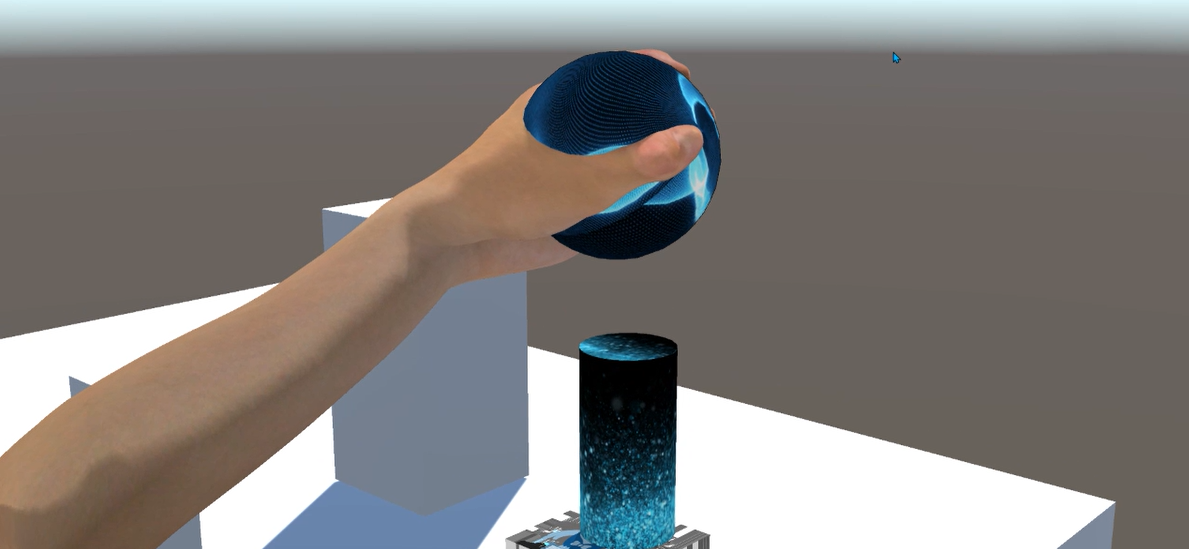
\includegraphics[width = \columnwidth]{figs/spheregrap2.png}
		\subcaption{保持状態}
		\end{minipage}
		\hspace{0.05\columnwidth}
		\begin{minipage}{0.4\columnwidth}
		\centering
		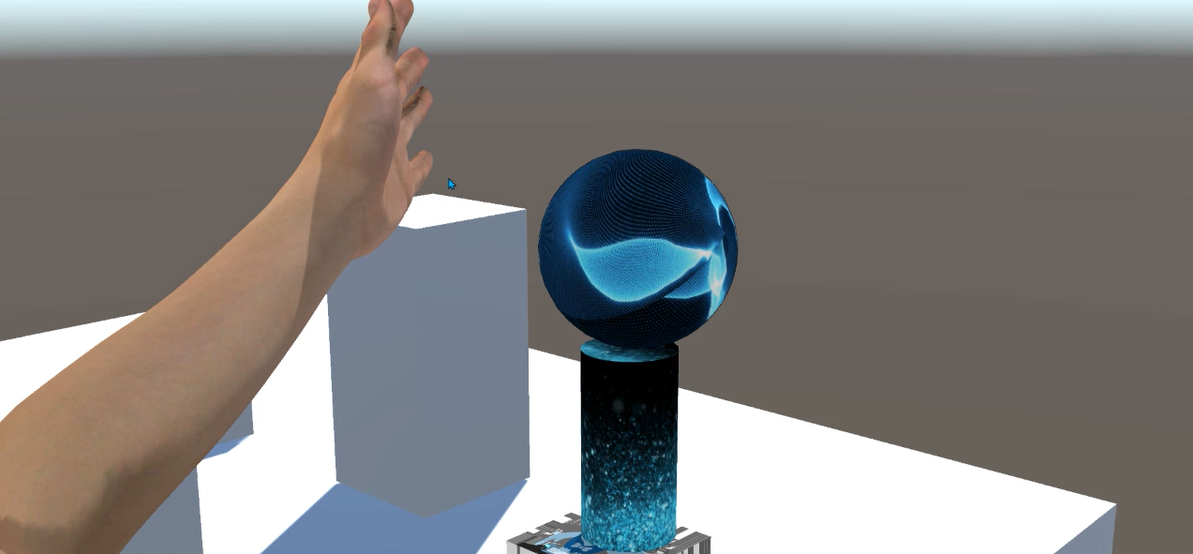
\includegraphics[width = \columnwidth]{figs/spherereleace.png}
		\subcaption{無保持状態}
		\end{minipage}
		\vspace{-10pt}
		\caption{仮想筋電義手モデルのオブジェクト保持}
		\label{fig:spheregrap}
		\end{figure}
		\vspace{-32pt}

\section{まとめと今後の課題}
	本研究では主に左腕切断者を想定した3Dモデルでトレーニングシステム
	を構成した.今後の課題としては,右腕切断者の場合の3Dモデルを用意する
	ことと,腕の動きをVR上に変換するためのインタフェースをマウスを用いて
	構成しているが,実際に上肢切断者を対象としてシミュレータを扱う場合,
	マウスを使用できないことを考慮し,光変位センサ「First VR」を用いた
	インタフェース改善や動作環境による入力遅延や誤差の改善,適切なトレーニング
	システムの構築および検討を行う予定である.
\vspace{-12pt}

\begin{thebibliography}{99}%参考文献
	\begin{spacing}{0.8}

	\bibitem{ref:1}
	芝軒 太郎 他.``VRを利用した筋電義手操作トレーニング
	システムの開発と仮想 Box and Block Test の実現''. 
	JRSJ. 2012 July.

	\bibitem{ref:2}
	Osumi M, et al.
	``Characteristics of Phantom Limb Pain Alleviated 
	with Virtual Reality Rehabilitation''. 
	Pain Med. 2019 May.

	\end{spacing}
\end{thebibliography}
\end{document}